\newpage
\section{Annexes}
\subsection{Exemples de débogage}

\begin{figure}[H]
    \begin{subfigure}{0.5\textwidth}
        \centering
        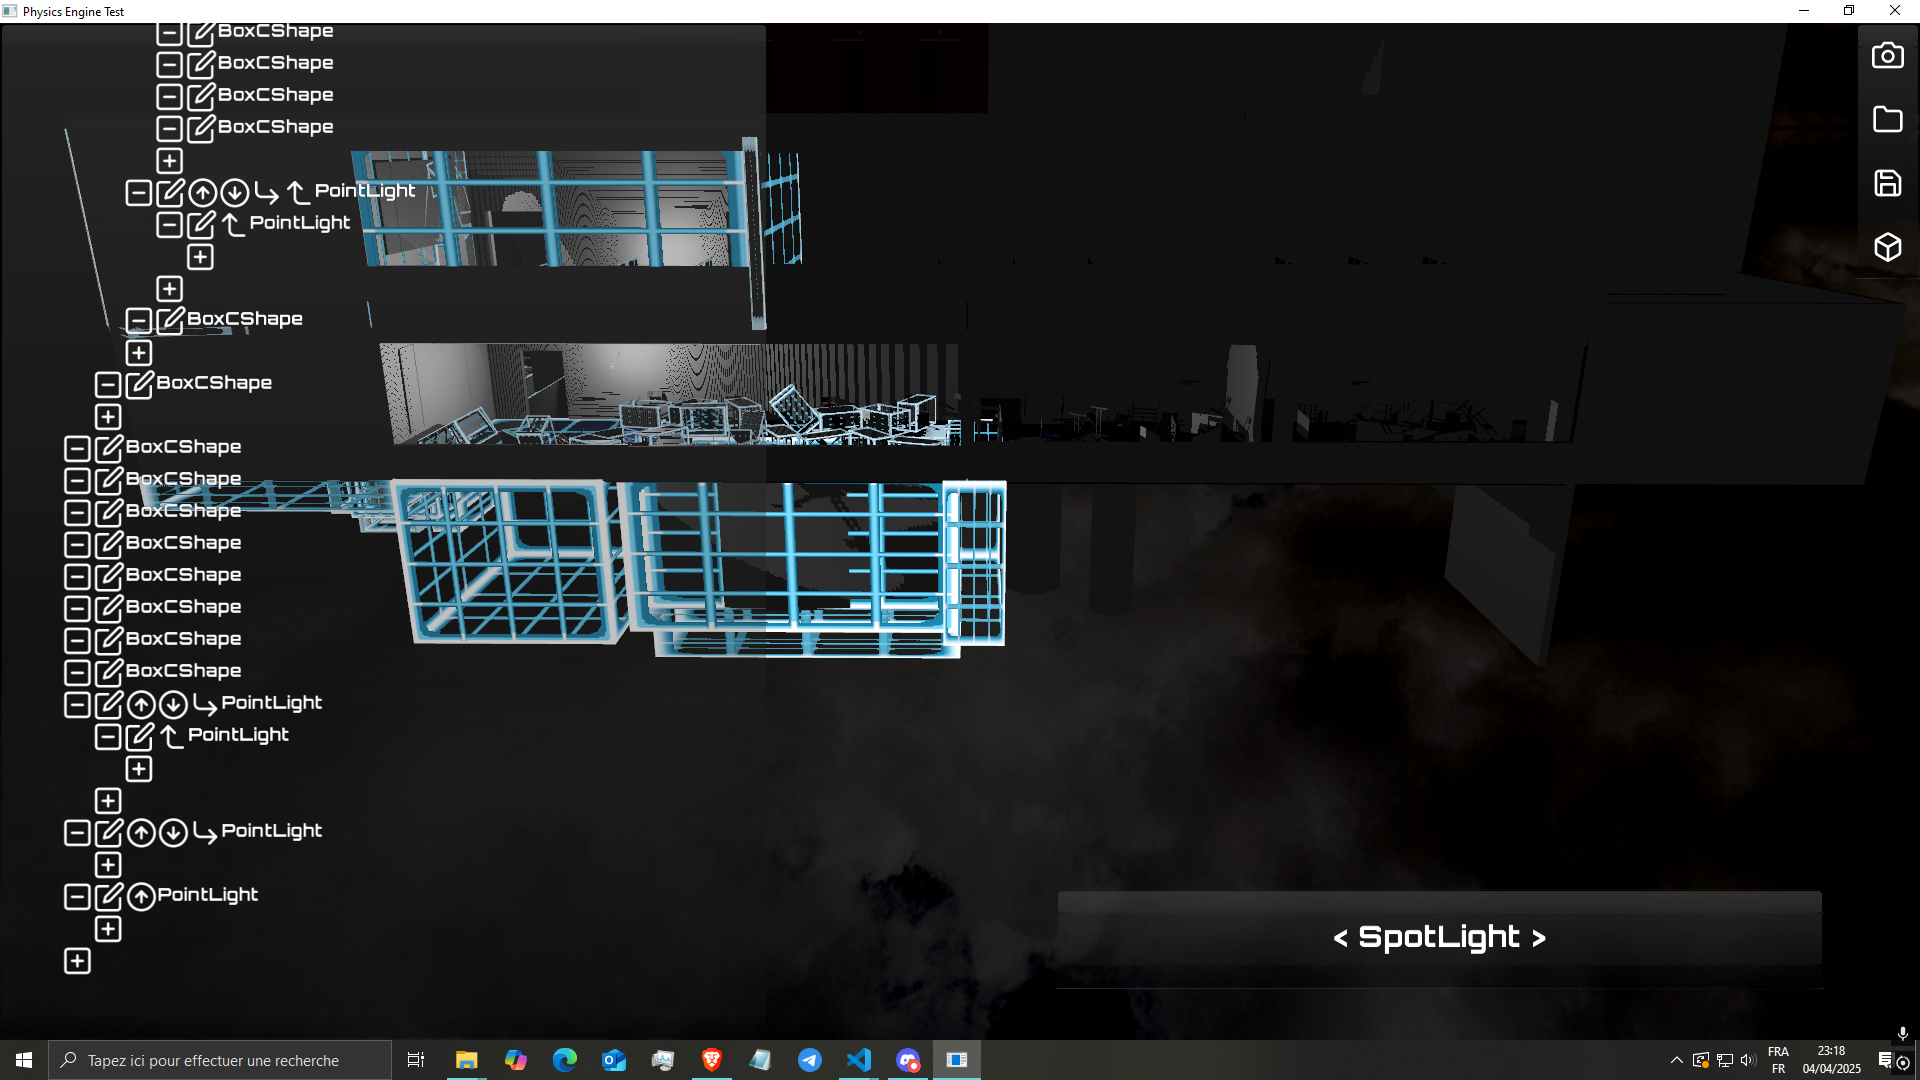
\includegraphics[width=0.8\textwidth]{images/gdb_editeur.png}
        \caption{Bug de collision}
        \label{fig:editeur1}
    \end{subfigure}
    \begin{subfigure}{0.5\textwidth}
        \centering
        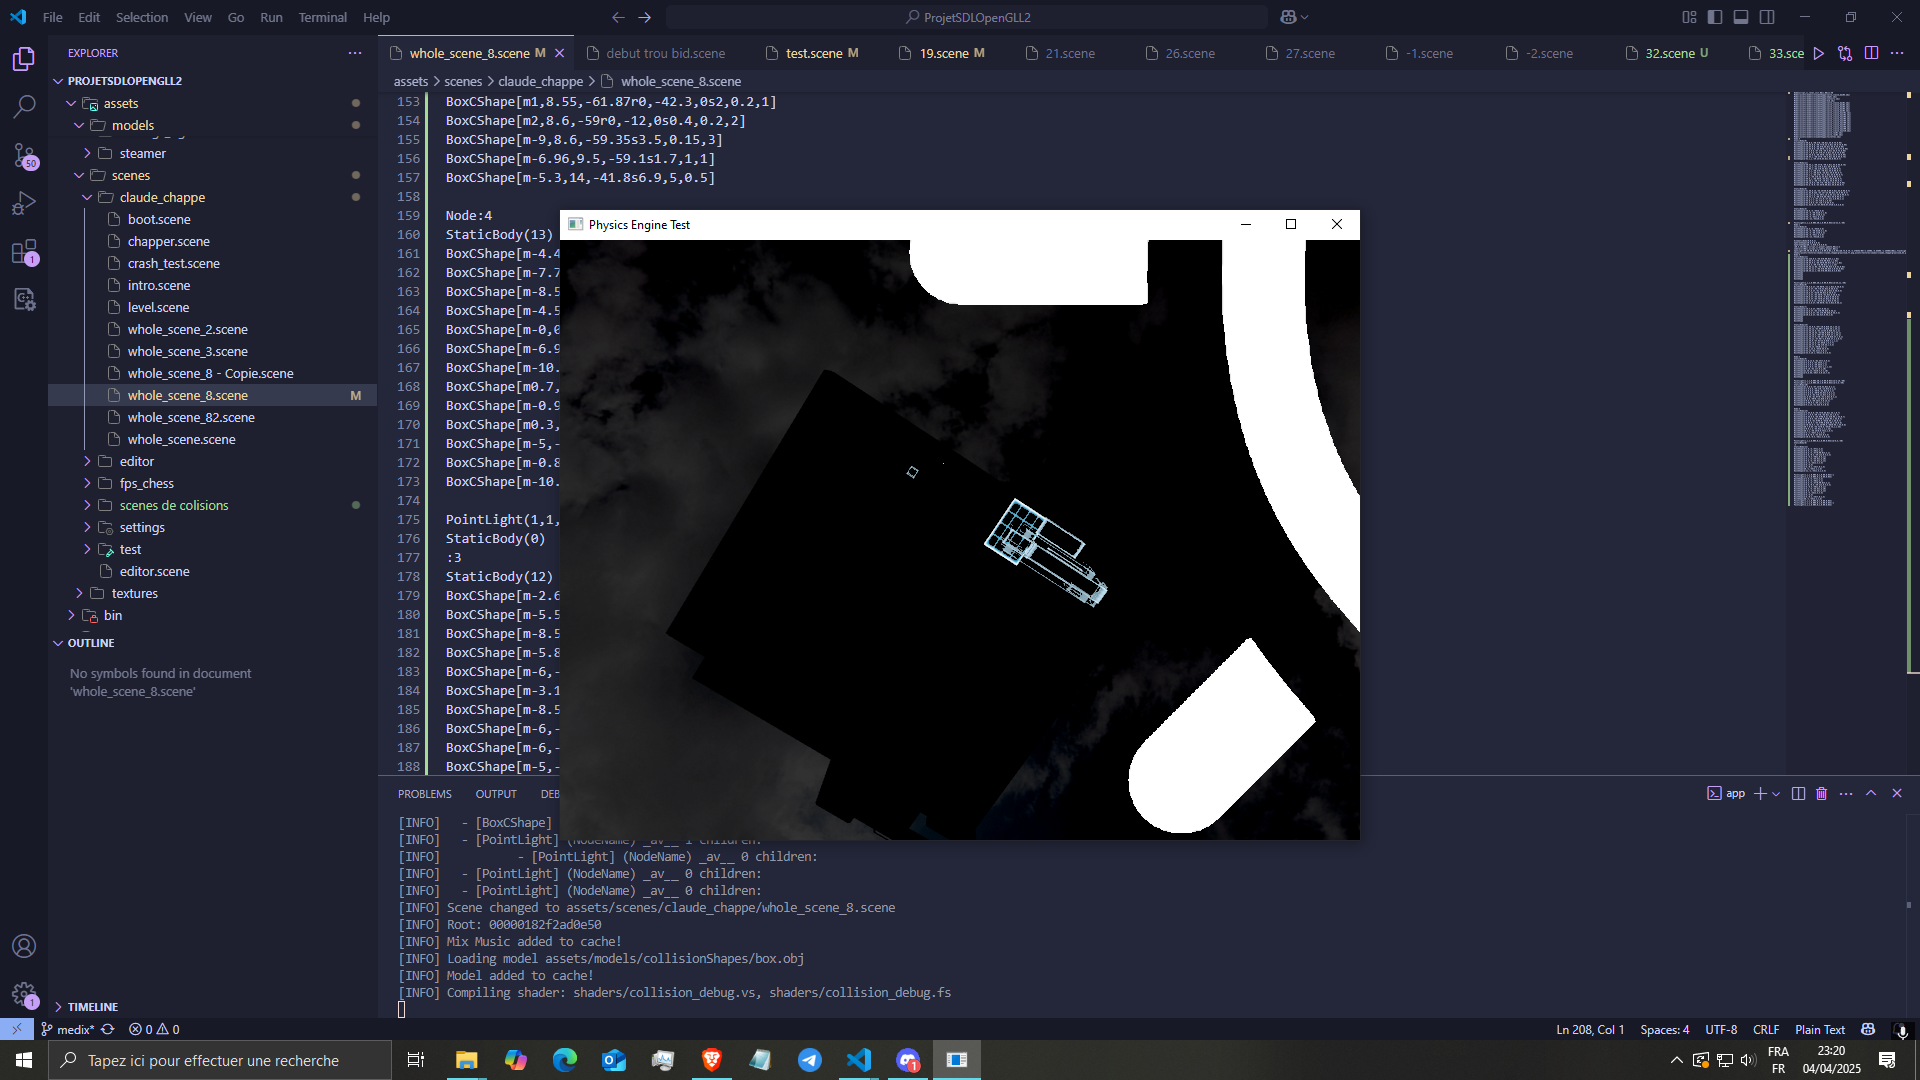
\includegraphics[width=0.8\textwidth]{images/gdb_editeur2.png}
        \caption{Bug de collision}
        \label{fig:editeur2}
    \end{subfigure}
    \begin{subfigure}{0.5\textwidth}
        \centering
        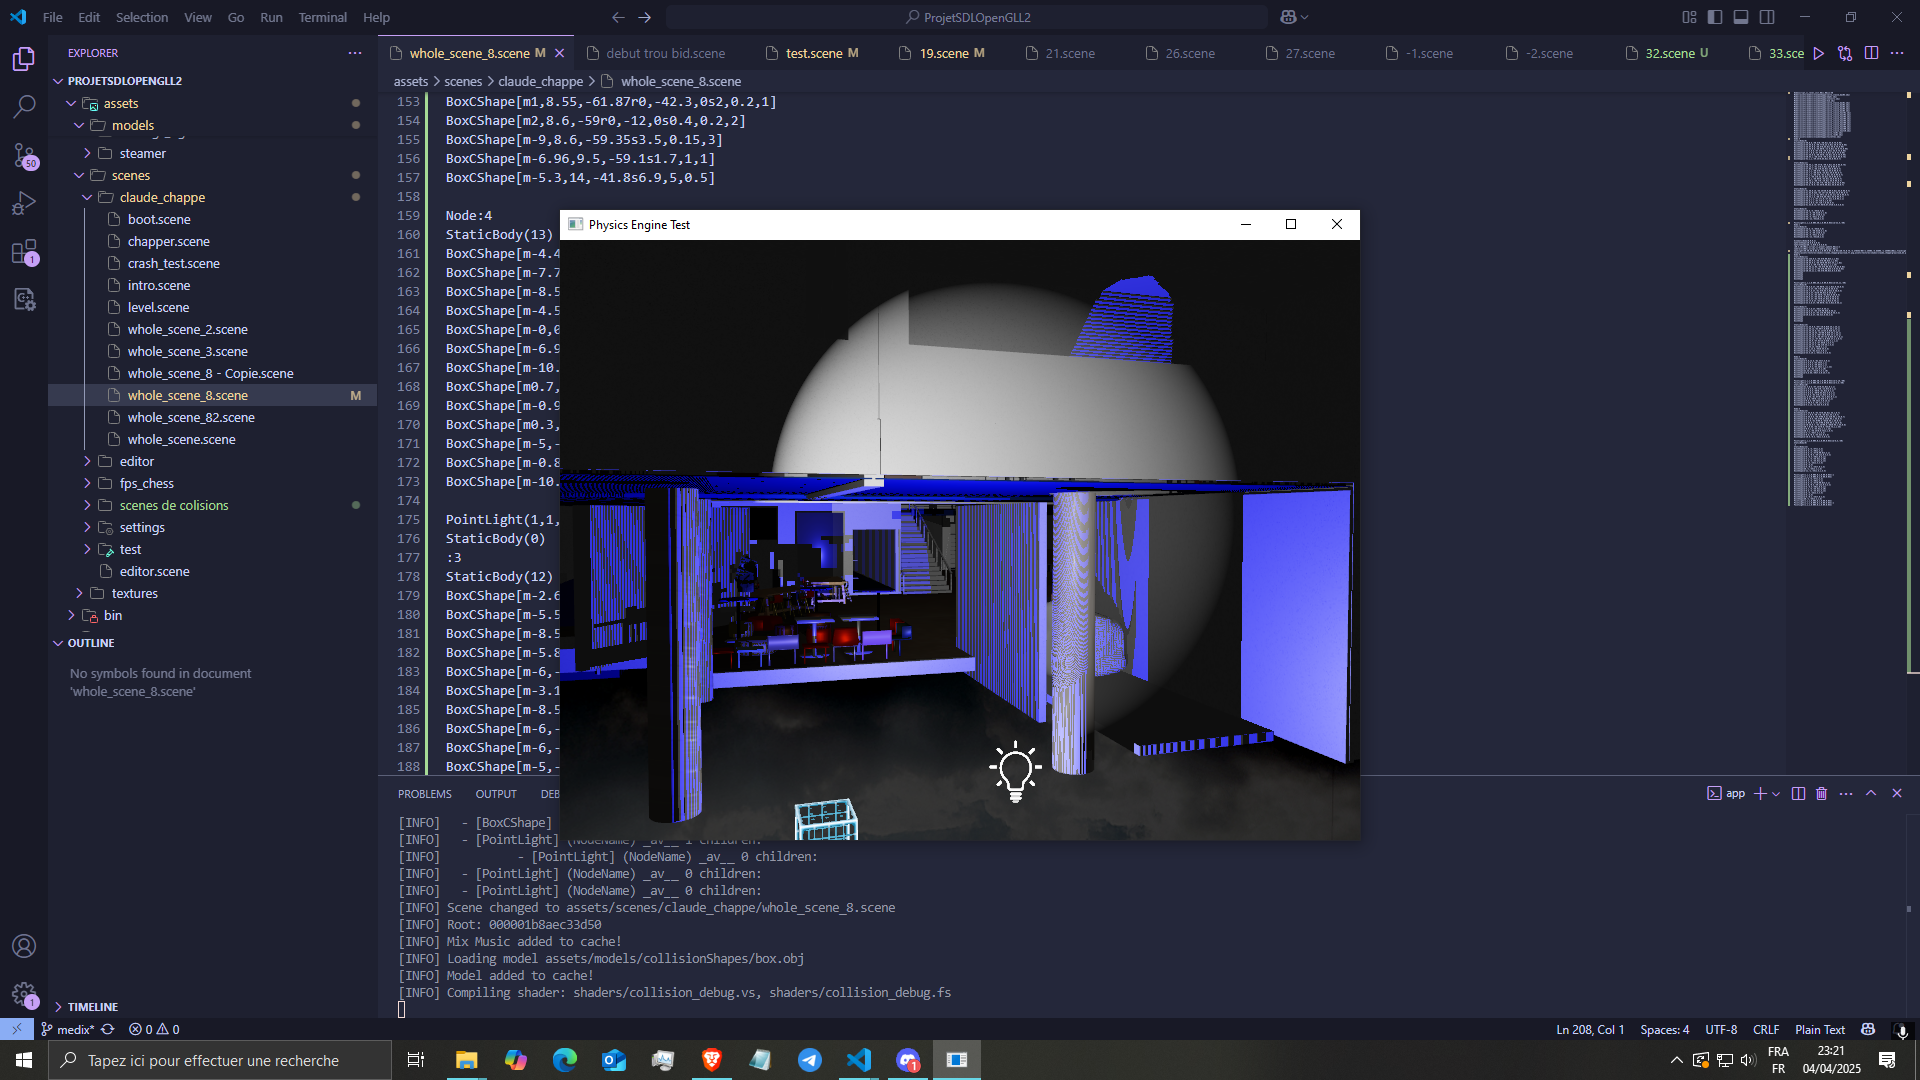
\includegraphics[width=0.8\textwidth]{images/gdb_editeur3.png}
        \caption{Bug d'affichage}
        \label{fig:editeur3}
    \end{subfigure}
    \caption{Exemples de bug à déboguer}
    \label{fig:debug}
\end{figure}

\begin{multicols}{2}
\begin{figure}[H]
    \centering
    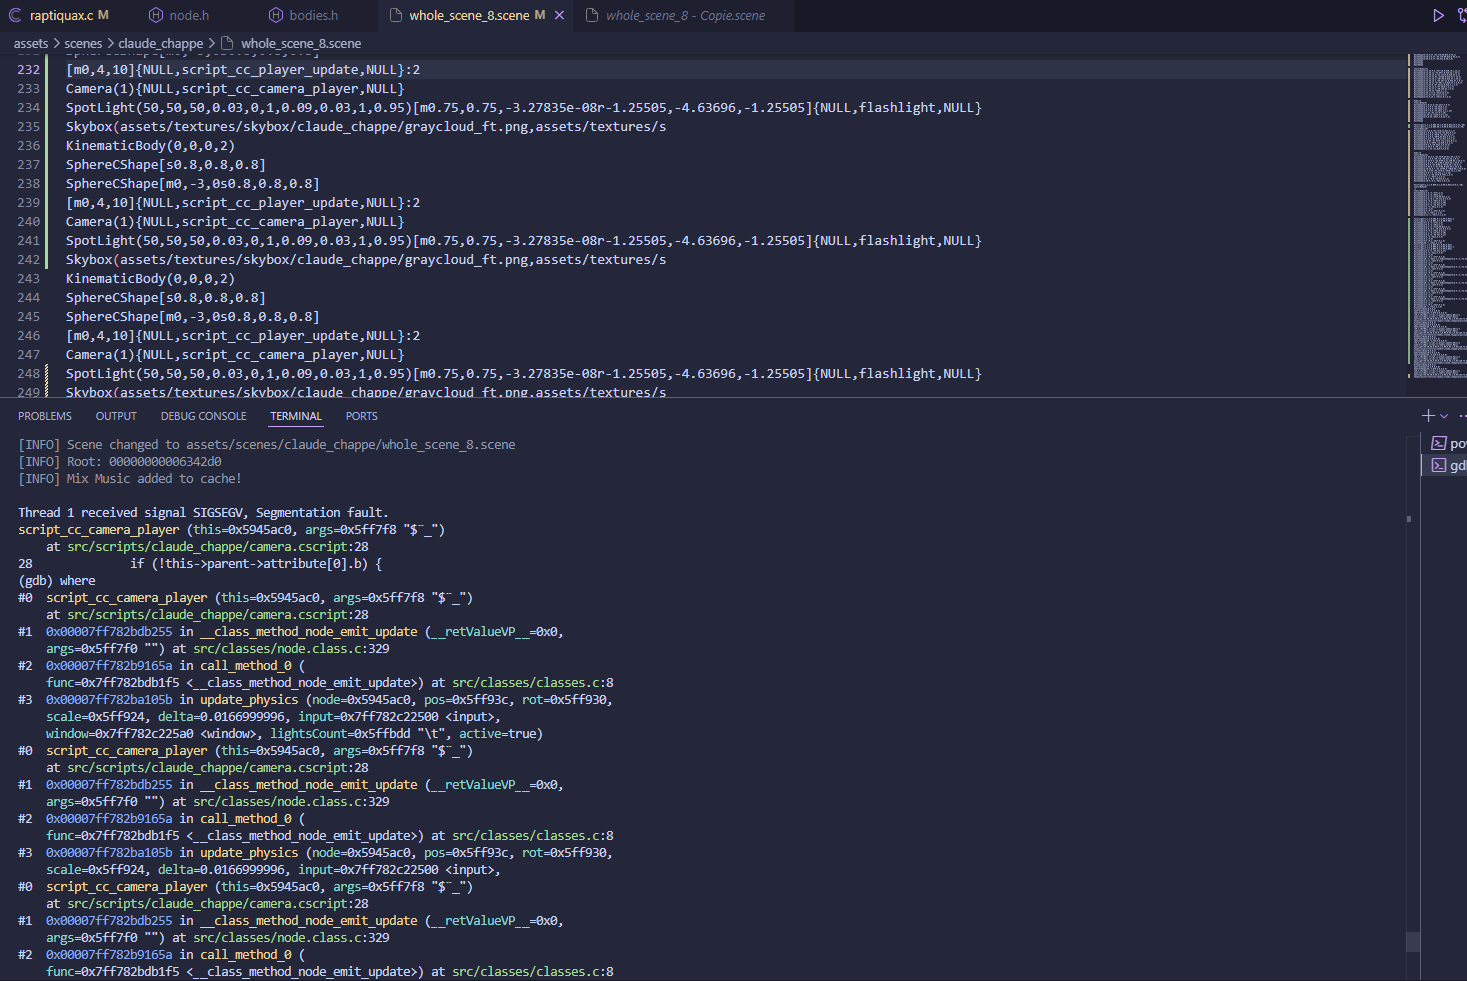
\includegraphics[width=0.5\textwidth]{images/gdb.png}
    \caption{Exemple de débogage avec GDB}
    \label{fig:debug}
\end{figure}

\begin{figure}[H]
    \centering
    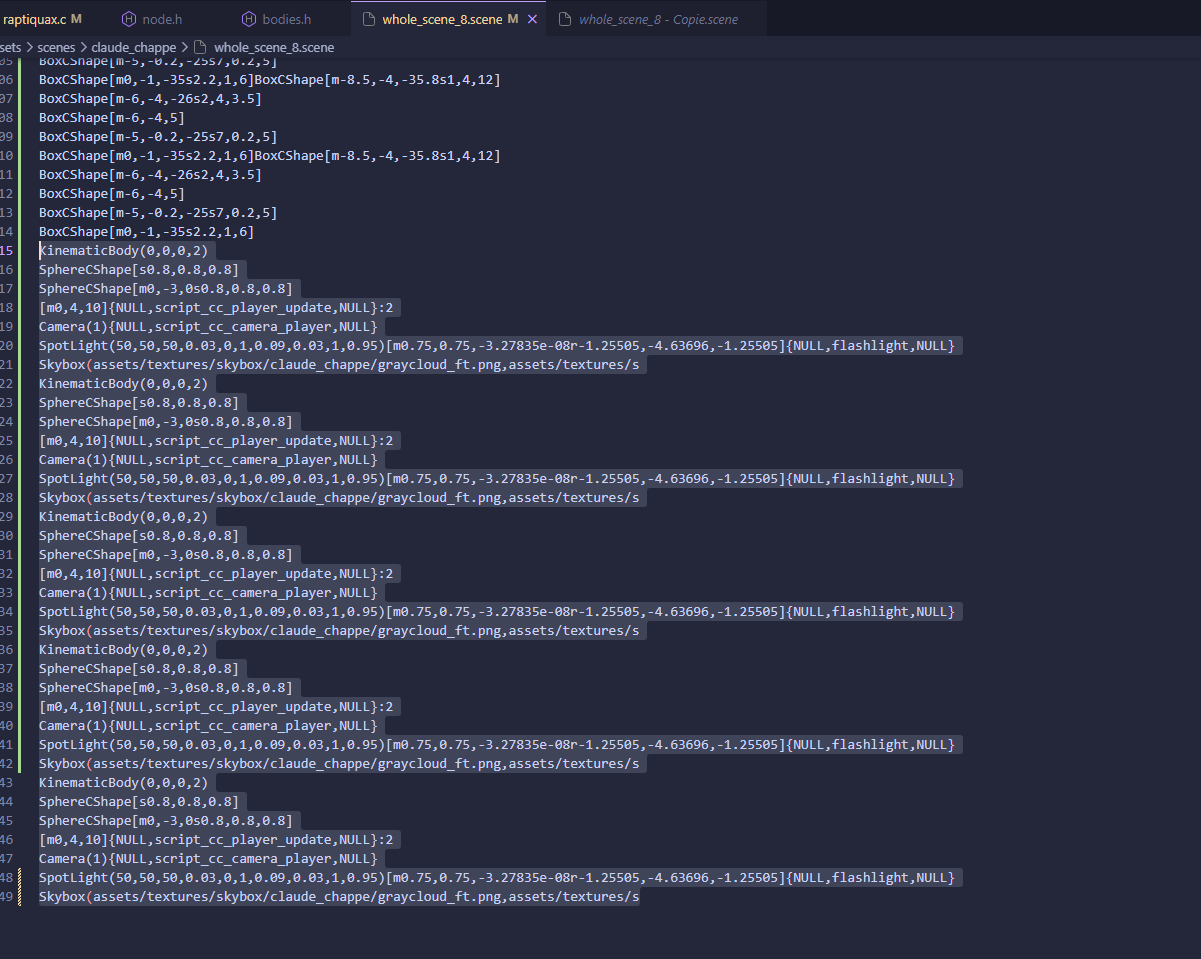
\includegraphics[width=0.5\textwidth]{images/gdb_fix.png}
    \caption{Correction du bug grâce à GDB}
    \label{fig:fix}
\end{figure}
\end{multicols}

\subsection{Code d'une classe générique}
\lstinputlisting[style=class_c,caption={Template de classe dans RaptiquaX},label=lst:class_template]{pages/developpement/class_templace.class.c}
\subsection{Rendu différé}
\label{sec:deferred_rendering}
Exemple de rendu différé :
\begin{figure}[h]
    \begin{subfigure}{0.5\textwidth}
        \centering
        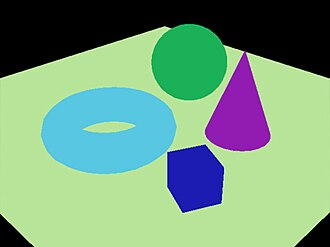
\includegraphics[width=0.8\textwidth]{images/Deferred_rendering_pass_col.jpg}
        \caption{G-Buffer de couleur}
        \label{fig:drendering_pass_col}
    \end{subfigure}
    \begin{subfigure}{0.5\textwidth}
        \centering
        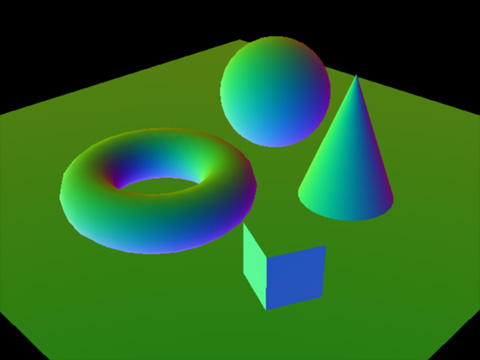
\includegraphics[width=0.8\textwidth]{images/Deferred_rendering_pass_nor.jpg}
        \caption{G-Buffer de normal}
        \label{fig:drendering_pass_normal}
    \end{subfigure}
    \begin{subfigure}{0.5\textwidth}
        \centering
        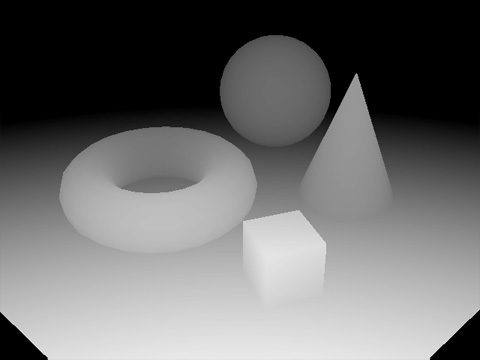
\includegraphics[width=0.8\textwidth]{images/Deferred_rendering_pass_dep.jpg}
        \caption{Z-Buffer}
        \label{fig:drendering_pass_depth}
    \end{subfigure}
    \begin{subfigure}{0.5\textwidth}
        \centering
        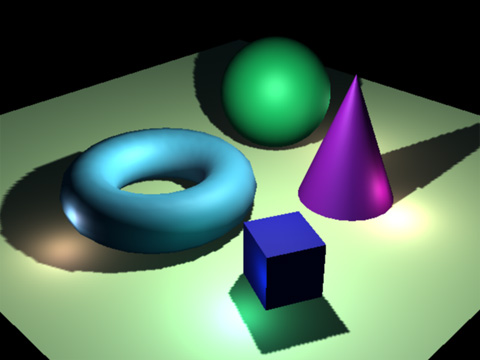
\includegraphics[width=0.8\textwidth]{images/Deferred_rendering_pass_res.jpg}
        \caption{Résultat final}
        \label{fig:drendering_result}
    \end{subfigure}
    \caption{Rendu différé d'une scène de volumes simples}
    \label{fig:defferred_rendering}
\end{figure}

\emph{Ici les Buffers ont été séparés pour montrer les différentes étapes du rendu différé.}

Le rendu différé s'appuie sur un G-Buffer qui contient les informations de la scène,
comme la couleur, les normaux et la profondeur. Ce G-Buffer est calculé en amont, lors
du rendu de la scène. C'est ensuite lors du rendu de la lumière et des effets de
post-processing qu'on utilise ce G-Buffer pour éviter de recalculer les informations de
la scène.
\newpage
\subsection{Pipeline graphique}
    \label{sec:graphics_pipeline}
    \begin{figure}[H]
        \begin{subfigure}{0.5\textwidth}
            \centering
            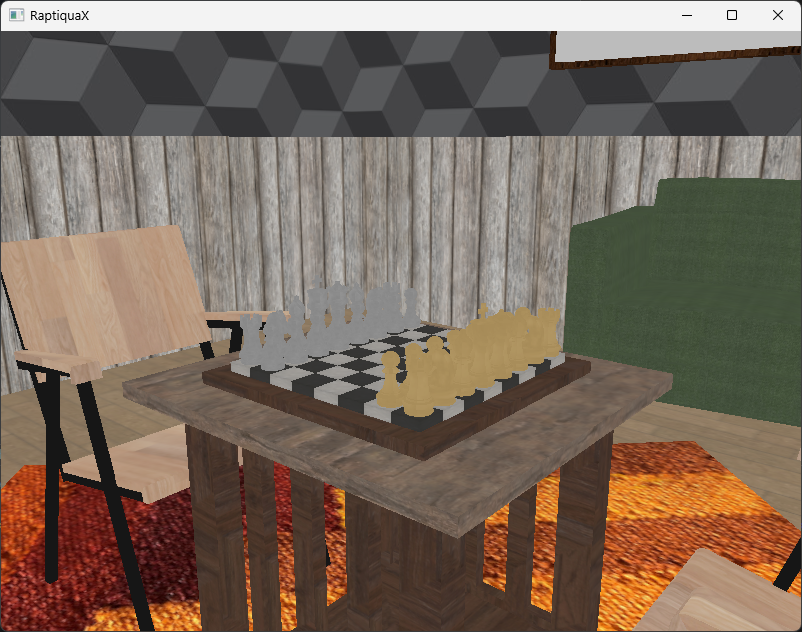
\includegraphics[width=0.8\textwidth]{images/raptiquax_rendering_gbuffer_albedo.png}
            \caption{G-Buffer de couleur}
            \label{fig:graphics_pipeline_gbuffer_albedo}
        \end{subfigure}
        \begin{subfigure}{0.5\textwidth}
            \centering
            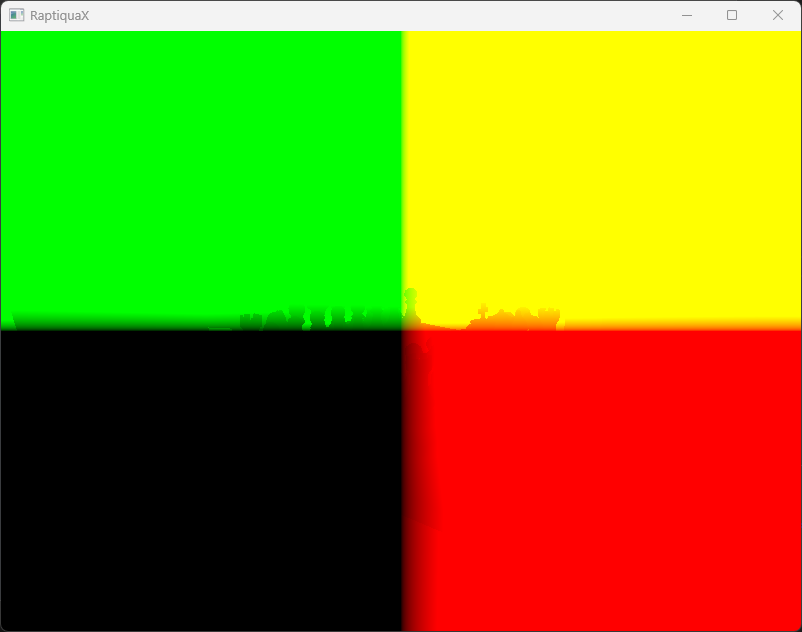
\includegraphics[width=0.8\textwidth]{images/raptiquax_rendering_gbuffer_position.png}
            \caption{G-Buffer de position}
            \label{fig:graphics_pipeline_gbuffer_position}
        \end{subfigure}
        \begin{subfigure}{0.5\textwidth}
            \centering
            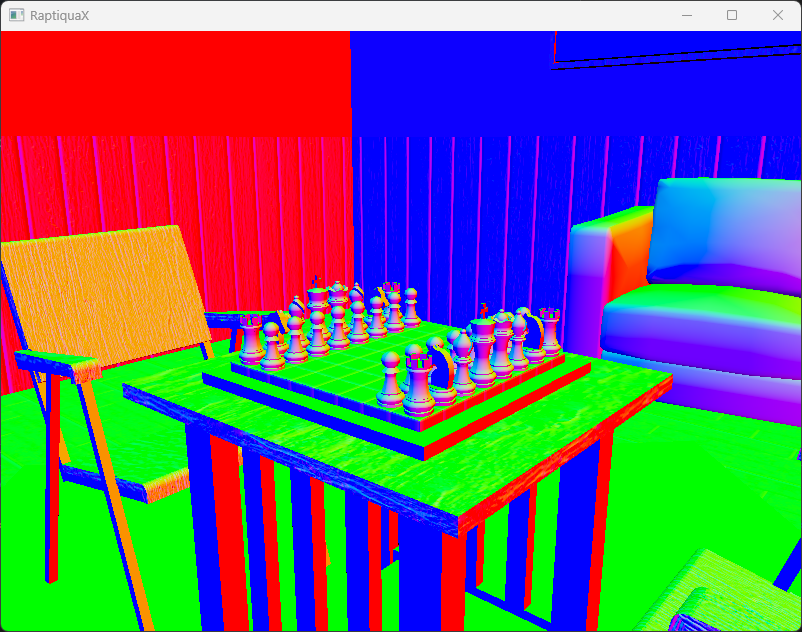
\includegraphics[width=0.8\textwidth]{images/raptiquax_rendering_gbuffer_normal.png}
            \caption{G-Buffer de normal}
            \label{fig:graphics_pipeline_gbuffer_normal}
        \end{subfigure}
        \begin{subfigure}{0.5\textwidth}
            \centering
            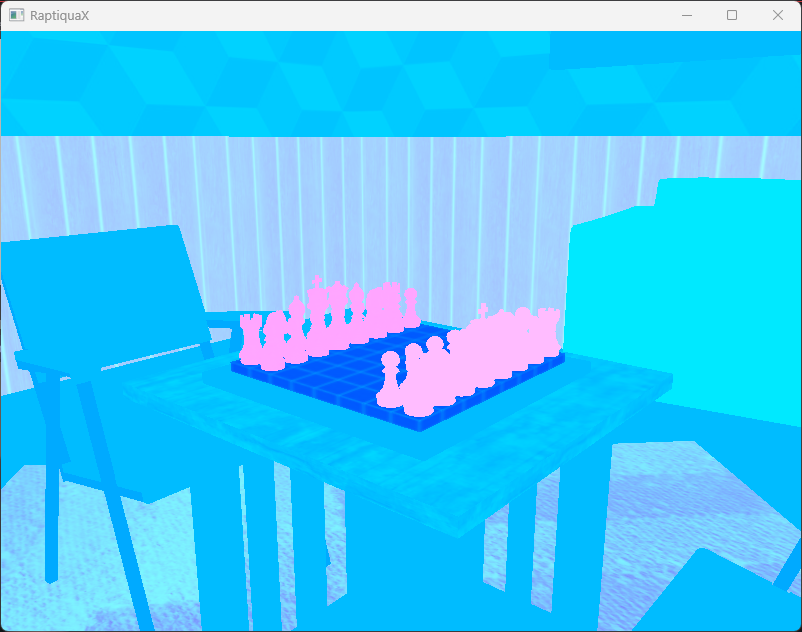
\includegraphics[width=0.8\textwidth]{images/raptiquax_rendering_gbuffer_extra.png}
            \caption{G-Buffer de métallicité et de rugosité}
            \label{fig:graphics_pipeline_gbuffer_color}
        \end{subfigure}
        \caption{G-Buffer de la scène}
        \label{fig:graphics_pipeline_gbuffer}
    \end{figure}
    \begin{figure}[H] 
        \begin{subfigure}{0.3\textwidth}
            \centering
            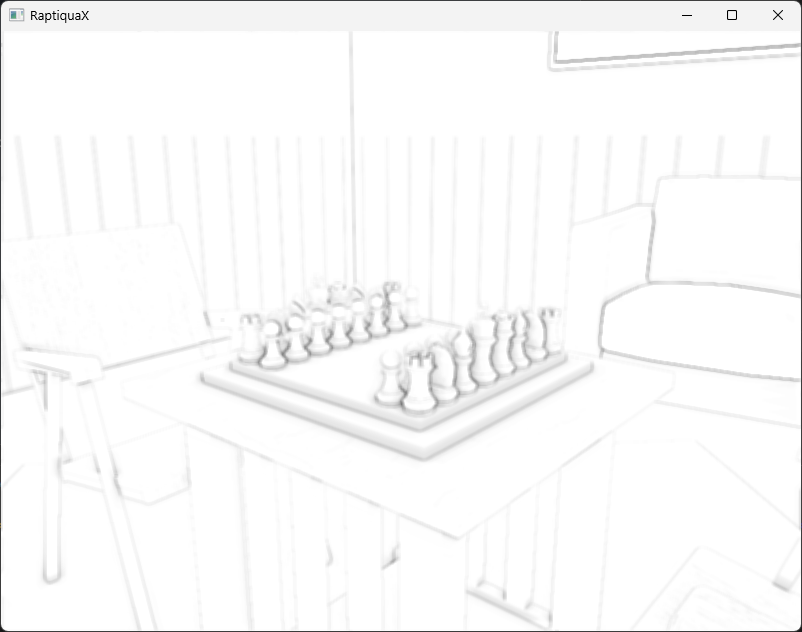
\includegraphics[width=0.8\textwidth]{images/raptiquax_rendering_ssao.png}
            \caption{Calque de l'occlusion ambiante}
            \label{fig:graphics_pipeline_gbuffer_ssao}
        \end{subfigure}
        \begin{subfigure}{0.3\textwidth}
            \centering
            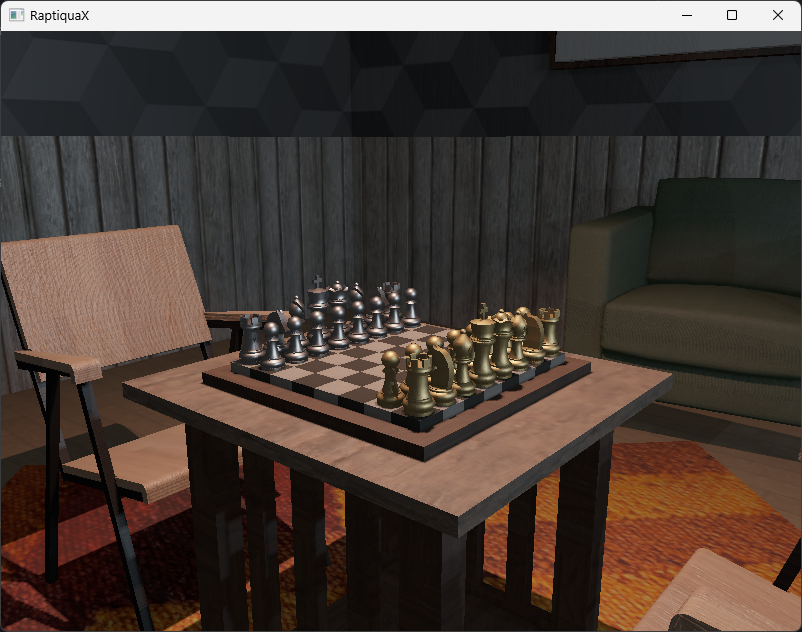
\includegraphics[width=0.8\textwidth]{images/raptiquax_rendering_lightings.png}
            \caption{Calque de la lumière et des ombres}
            \label{fig:graphics_pipeline_gbuffer_light}
        \end{subfigure}
        \begin{subfigure}{0.3\textwidth}
            \centering
            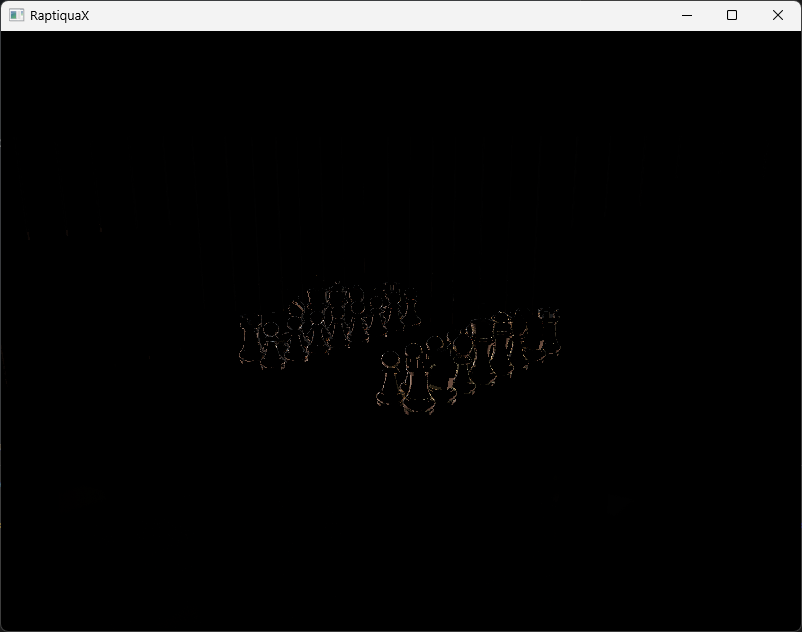
\includegraphics[width=0.8\textwidth]{images/raptiquax_rendering_ssr.png}
            \caption{Calque des réflexion et reflets}
            \label{fig:graphics_pipeline_gbuffer_ssr}
        \end{subfigure}
        \begin{subfigure}{0.3\textwidth}
            \centering
            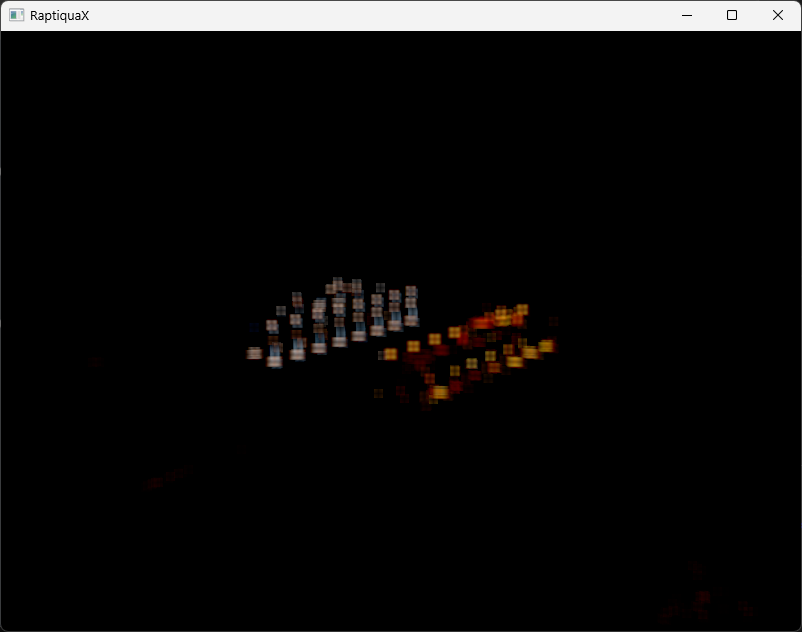
\includegraphics[width=0.8\textwidth]{images/raptiquax_rendering_bloom.png}
            \caption{Calque de l'éblouissement}
            \label{fig:graphics_pipeline_gbuffer_bloom}
        \end{subfigure}
        \begin{subfigure}{0.3\textwidth}
            \centering
            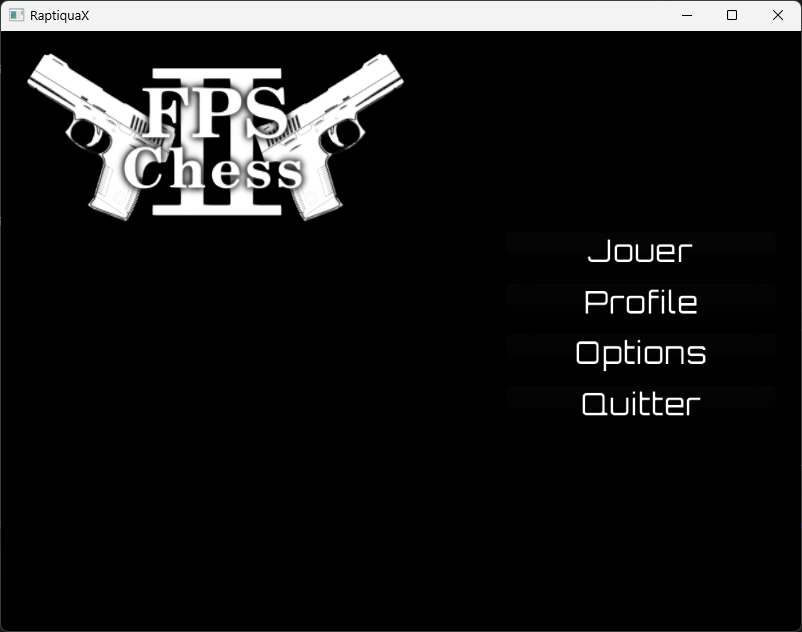
\includegraphics[width=0.8\textwidth]{images/raptiquax_rendering_gui.png}
            \caption{Calque de l'interface utilisateur}
            \label{fig:graphics_pipeline_gbuffer_gui}
        \end{subfigure}
        \caption{Calques de la scène}
        \label{fig:graphics_pipeline_post_processing}
    \end{figure}
    \begin{figure}[H]
        \centering
        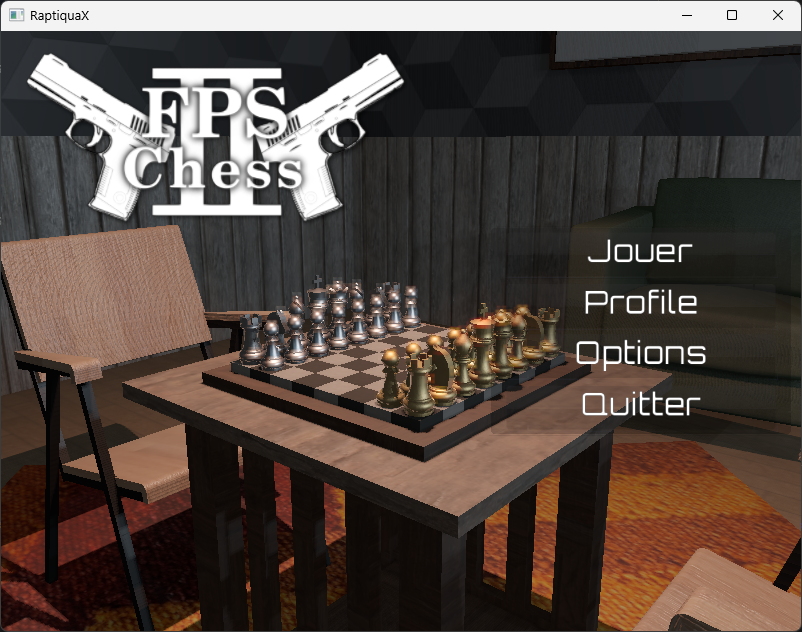
\includegraphics[width=0.5\textwidth]{images/raptiquax_rendering_result.png}
        \caption{Résultat de la pipeline graphique}
        \label{fig:graphics_pipeline_result}
    \end{figure}
\subsection{Musique}
\begin{figure}[H]
    \centering
    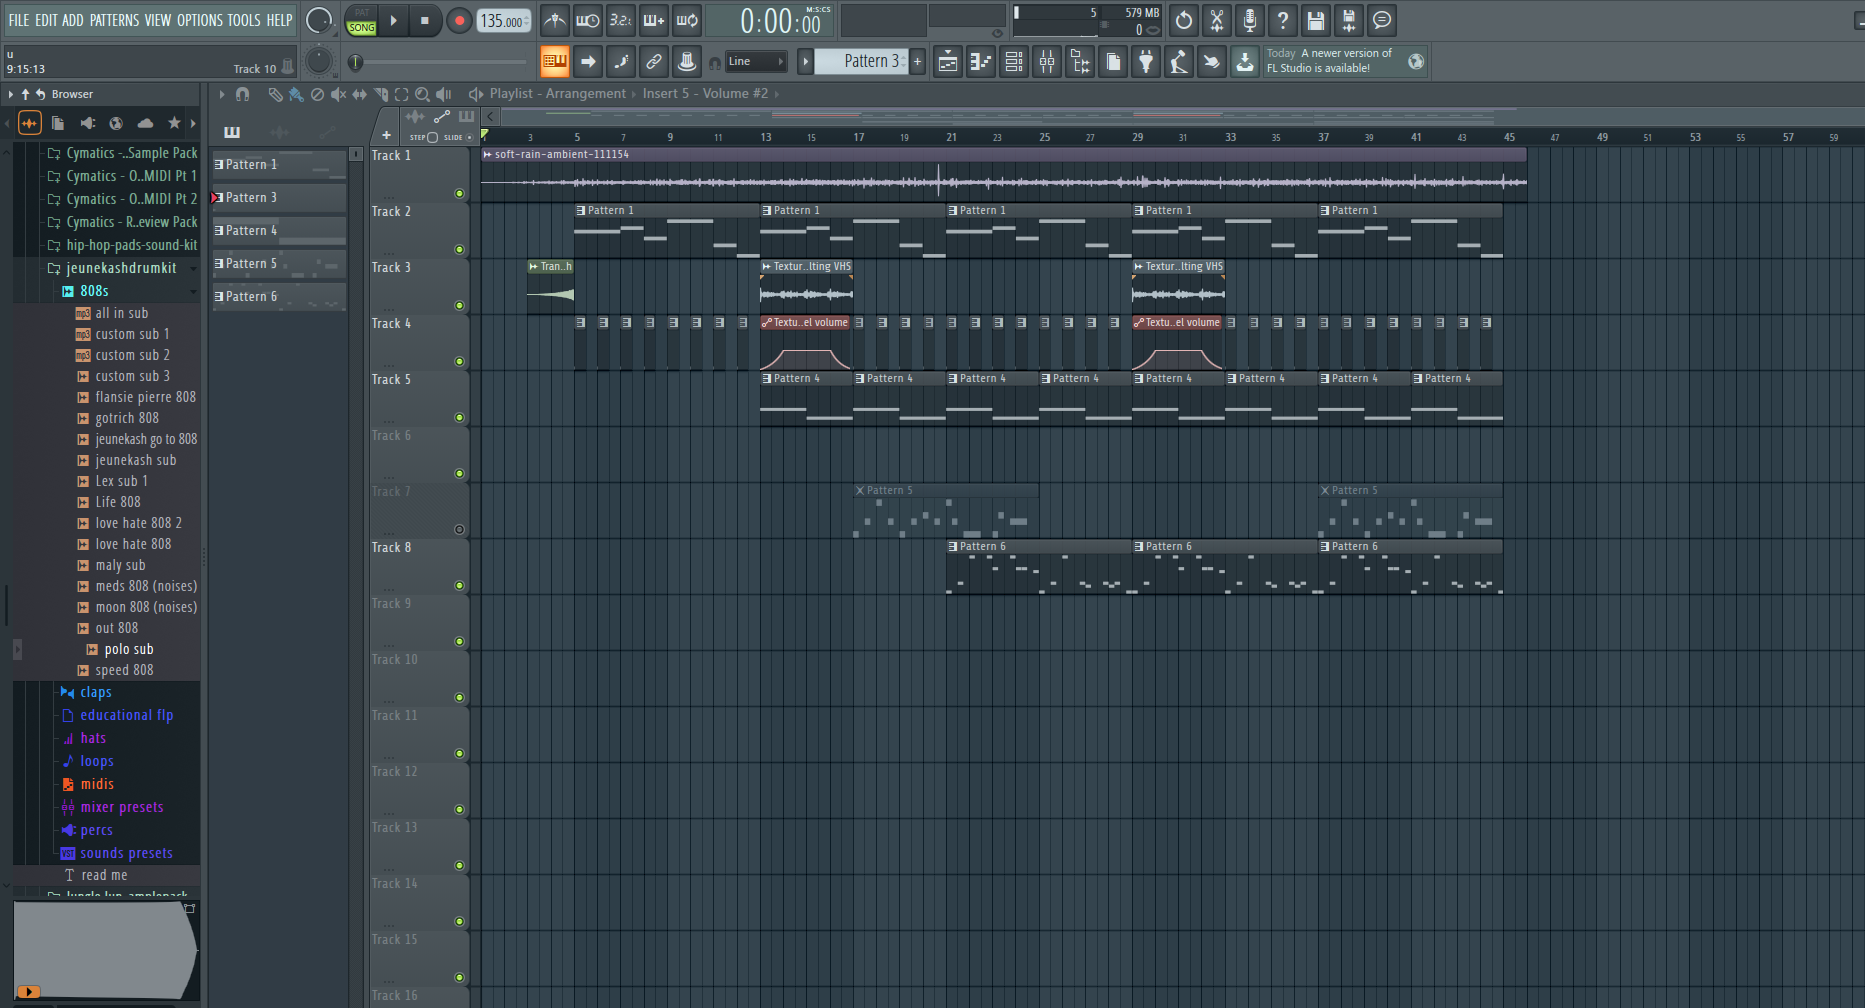
\includegraphics[width=1\linewidth]{images/flstudio.png}
    \caption{fl studio}
    \label{fig:flstudio.png}
\end{figure}

\newpage
\subsection{Tableau des différents n\oe{}uds de la scène}
    \renewcommand{\arraystretch}{1.2}
    \setlength{\tabcolsep}{10pt}

    \begin{longtable}{>{\bfseries}p{0.25\linewidth} p{0.7\linewidth}}
        \toprule
        \textbf{Nœud} & \textbf{Description} \\
        \midrule
        Node & Classe de base pour tous les objets de la scène \\
        Camera & Représente un point de vue pour le rendu \\
        BoxCShape & Forme de collision en boîte \\
        CapsuleCShape & Forme de collision en capsule \\
        CShape & Classe de base des formes de collision \\
        MeshCShape & Forme de collision basée sur un maillage \\
        PlaneCShape & Plan infini utilisé pour les collisions \\
        RayCShape & Détecteur de collision basé sur un rayon \\
        SphereCShape & Forme de collision sphérique \\
        Button & Élément d'interface cliquable \\
        CheckBox & Case à cocher \\
        ControlFrame & Conteneur pour organiser l'interface \\
        Frame & Conteneur de base pour l'interface \\
        ImageFrame & Cadre affichant une image \\
        InputArea & Champ de saisie de texte \\
        Label & Étiquette de texte \\
        SelectList & Liste déroulante ou défilable \\
        Slider & Curseur pour sélectionner une valeur \\
        DirectionalLight & Source lumineuse directionnelle (\textit{ex : soleil}) \\
        Light & Classe de base pour les sources de lumière \\
        PointLight & Lumière omnidirectionnelle ponctuelle \\
        SpotLight & Source lumineuse en forme de cône \\
        Mesh & Maillage basique sans texture \\
        Model & Modèle 3D complet et texturé \\
        Area & Zone invisible déclenchant des événements \\
        Body & Classe de base pour les corps physiques \\
        KinematicBody & Corps physique contrôlé manuellement \\
        RigidBody & Objet physique entièrement simulé \\
        StaticBody & Corps physique immobile \\
        PhysicalNode & Base pour les nœuds liés à la physique \\
        RenderTarget & Sous scène rendu dans une texture \\
        Skybox & Cube d'environnement représentant le ciel \\
        TexturedMesh & Maillage avec textures appliquées \\
        \bottomrule
        \caption{Liste des n\oe{}uds de la scène}
        \label{tab:raptiquax_nodes}
    \end{longtable}

\subsection{Tableau des commandes Socket du mini-jeu \og FPS Chess \fg{}}
    \begin{table}[H]
        \centering
        \scriptsize
        \renewcommand{\arraystretch}{1.1}
        \begin{tabular}{|l|p{2.5cm}|p{4.5cm}|}
            \hline
            \textbf{Commande} & \textbf{Arguments} & \textbf{Description} \\
            \hline
            PONG & Aucun & Répond au ping du serveur. \\
            LOGIN & Nom d'utilisateur & Authentifie l'utilisateur et enregistre son nom. \\
            CREATE\_PARTY & Nom de la partie & Crée une nouvelle partie avec un nom donné. \\
            LIST\_PARTY & Aucun & Liste les parties existantes. \\
            EXIT\_PARTY & Aucun & Quitte la partie actuelle. \\
            JOIN\_PARTY & ID de la partie & Rejoint une partie donnée (par ID). \\
            RENAME\_PARTY & Nouveau nom & Renomme la partie actuelle. \\
            PARTY\_SET\_DATA & Clé=Valeur & Définit une valeur clé dans les données de la partie. \\
            PARTY\_GET\_DATA & Clé & Récupère une valeur clé des données de la partie. \\
            PARTY\_GET\_SELF\_INDEX & Aucun & Récupère l'index du joueur dans la partie. \\
            EXIT & Aucun & Déconnecte le client du serveur. \\
            G\_MSG & Message & Envoie un message global aux autres clients connectés. \\
            MSG & Message & Envoie un message à tous les joueurs de la partie ou globalement si hors partie. \\
            \hline
        \end{tabular}
        \caption{Requêtes gérées par le serveur SocketIO du moteur RaptiquaX}
        \label{tab:raptiquax_requests}
    \end{table}